In this section we present the comparison between the execution of some patterns
using hadoop and pig. The patterns considered for this preliminary analysis was
those ones are the same classification in \cite{White:2012} and
\cite{pig-designpattern:2014}. We chose three different design patterns to
proceed with the experiments. Following we describe the input data, the
execution configuration and the analysis of the produced results. 

\subsection{Input Data Description}
 
For our execution analysis we used the retrieved the open data from
\textit{stackexchange}\footnote{https://archive.org/details/stackexchange}. The
information from this site include data about users forum, with comments
about specific topics. 

\begin{table}\centering \small
\begin{tabular}{|l|l|l|} \hline
\textbf{Input Data Type}		& \textbf{Comments.xml} & \textbf{Users.xml}  \\
\hline\hline 
\textit{ebooks}			&   413.8 KB    &      827.8 KB				\\ \hline
\textit{webapps}		&   7.8 MB	    &      17.3 MB 				\\ \hline
\textit{wordpress}		&   42.1 MB	    &      13.8 MB				\\ \hline
\textit{tex}			&   99.4 MB 	&      15.4 MB			 	\\ \hline
\textit{serverfault}	&   158.8 MB	&      54.0 MB				\\ \hline
  
\end{tabular}
\caption{\label{table:input-data-length} Input Data Description.}
\end{table}

%From these data we executed the programs 
 
\subsection{Execution Description}
 
 We considered for the result value generated by the hadoop and pig environments
 for the analysis of the Jobs execution from the input data described in the
 previous section: \textit{Elapsed Time}, \textit{Average\footnote{The term
 \textit{Average} is because, most, if not all your map tasks and reduce tasks
 would be running in parallel.} Map Time}, \textit{Average Suffle Time} and
 \textit{Average Reduce Time}.
  
\begin{itemize}
  \item \textbf{\textit{Elapsed Time}} -  It is the time taken from start of
  the execution Job to the end. Elapsed time includes I/O time and all
  other types of wait.
  \item \textbf{\textit{Average Map Time}} - It is the first phase, where each Map task is provided
  with an input split, which is a small portion of the total input data. The Map
  tasks process data from the input and output intermediate data which
  needs to go to the reducers.
  \item \textbf{\textit{Average Suffle Time}} - It is the step where the
  intermediate data that was generated by Map tasks is directed to the correct reducers. Reducers usually handle a
  subset of the total number of keys generated by the Map task. The Shuffle
  phase assigns keys to reducers and sends all values pertaining to a key to the
  assigned reducer. Sorting (or Merging) is also a part of this phase, where
  values of a given key are sorted and sent to the reducer. As you may realize,
  the shuffle phase involves transfer of data across the network from Map to
  Reduce tasks.       
  \item \textbf{\textit{Average Reduce Time}} - It is the last step of the
  MapReduce Job. The Reduce tasks process all values pertaining to a key and
  output their results to the desired location. 
\end{itemize}

All the execution\footnote{The execution were also made over a MacOS X Yosemite
Version 10.10.2; Processor Intel 2.8 GHz Core i5 and RAM Memory of 16GB 1600 MHz
DDR3.} were made using the Hortonworks\footnote{http://www.hortonworks.com}
virtual machine environment. 

\subsection{Results}          
   \begin{figure}[ht!]
 \centering 
  \subfloat[\textit{Ebooks} Data]
  {\label{fig:pisp6}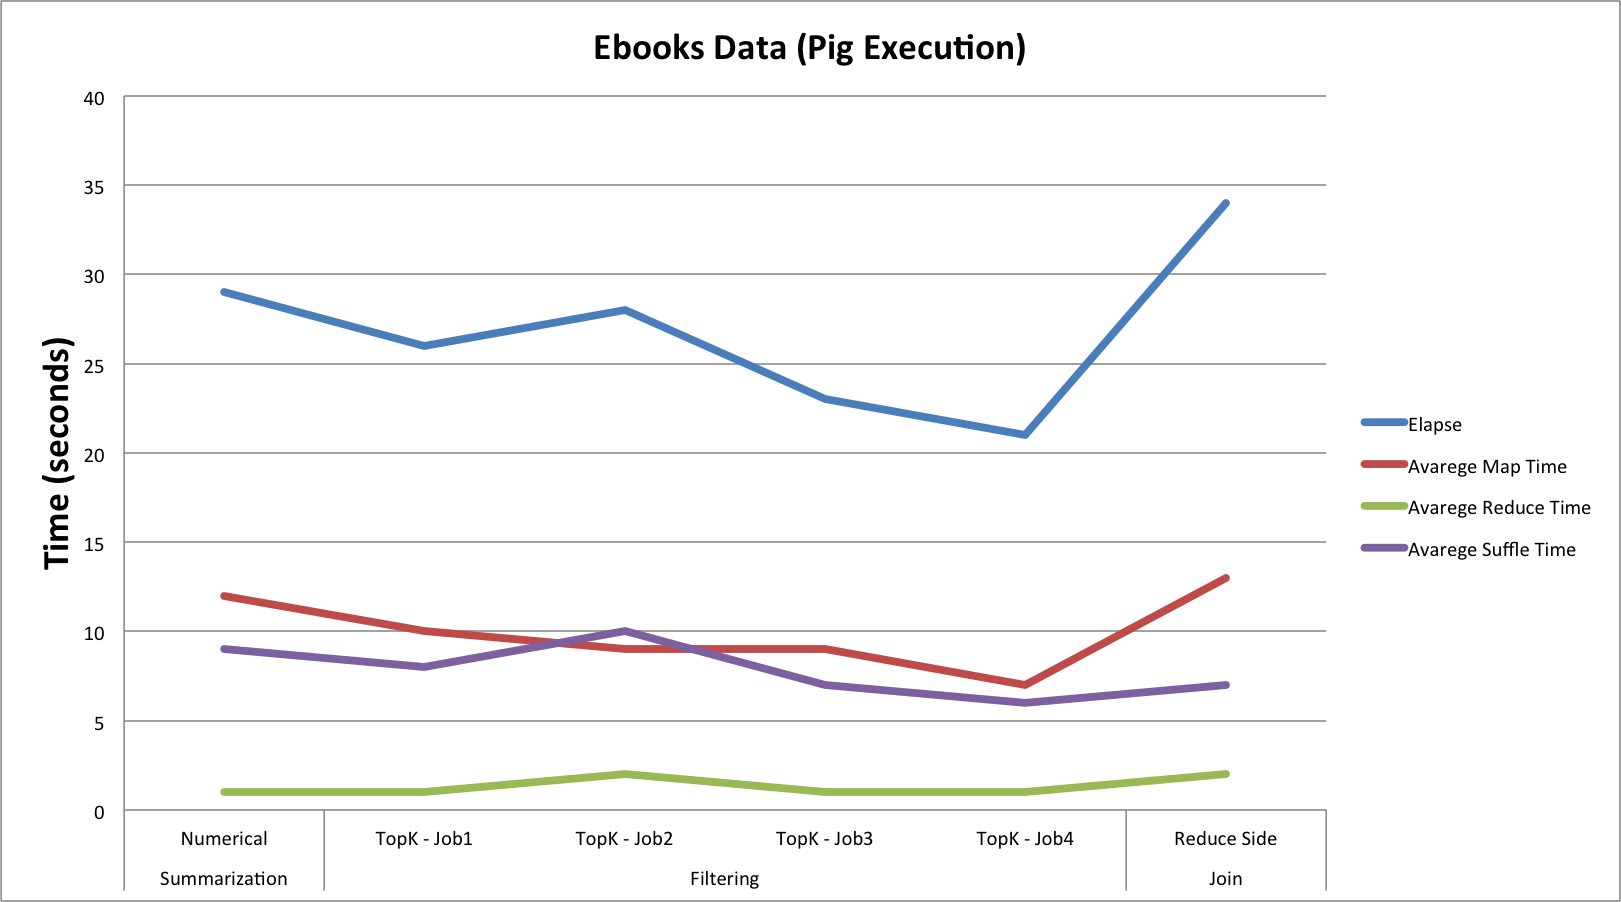
\includegraphics[width=0.471\textwidth]{figs/analysis-charts/pig/ebooks.png}}   
  \subfloat[\textit{Tex} Data]
  {\label{fig:pisp7}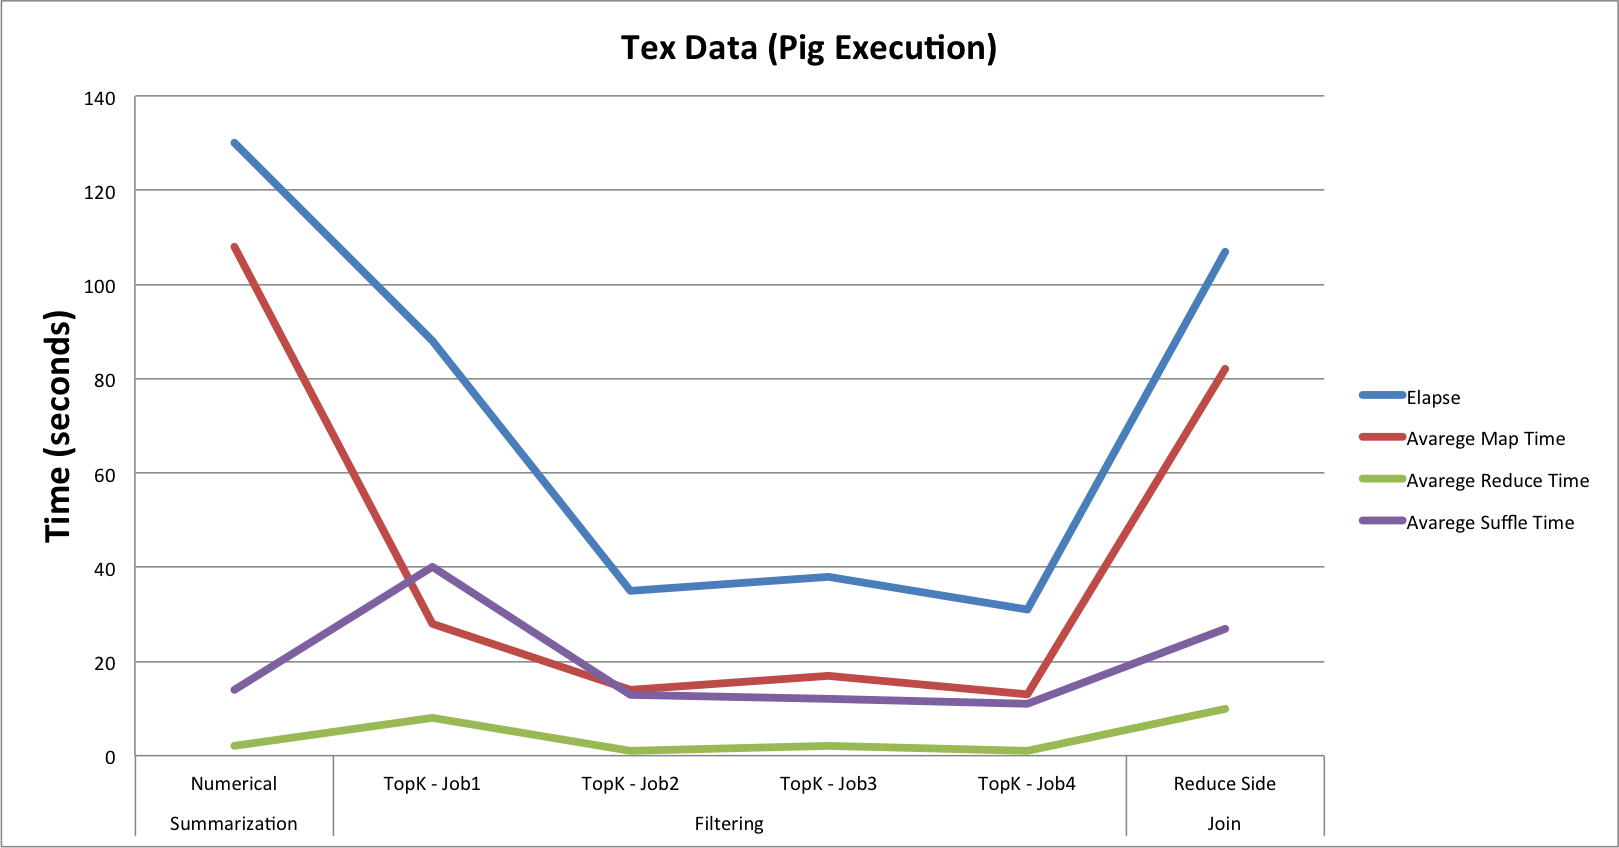
\includegraphics[width=0.5\textwidth]{figs/analysis-charts/pig/tex.png}}
   %add desired spacing between images, e. g. ~, \quad, \qquad etc. (or a blank line to force the subfig onto a new line)
  %~
  \\
  \subfloat[\textit{Serverfault} Data]
  {\label{fig:pisp6}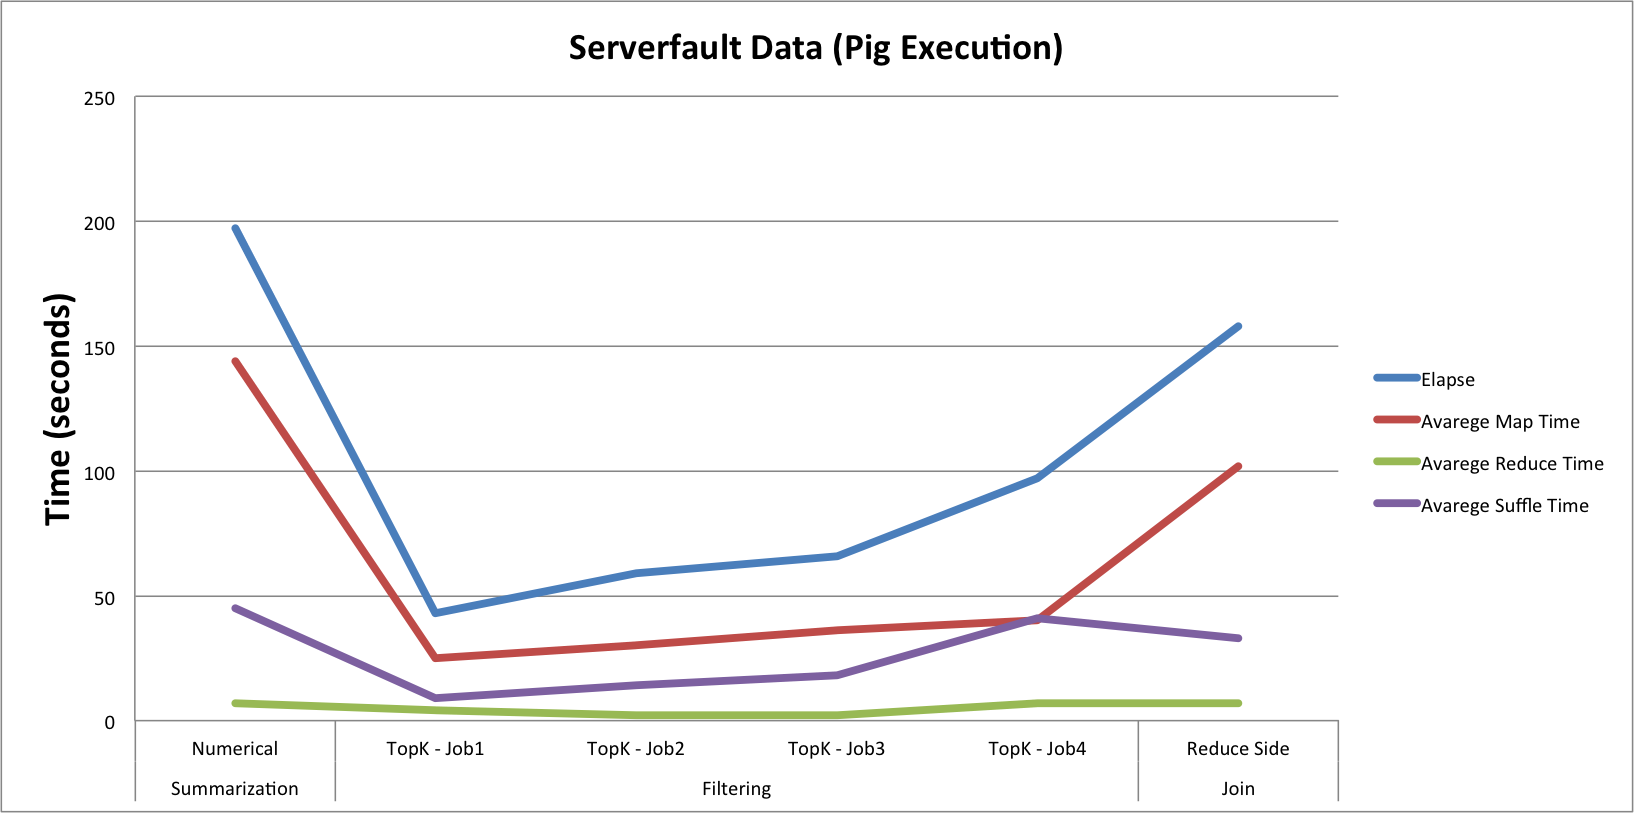
\includegraphics[width=0.5\textwidth]{figs/analysis-charts/pig/serverfault.png}}   
  \subfloat[\textit{Wordpress} Data]
  {\label{fig:pisp7}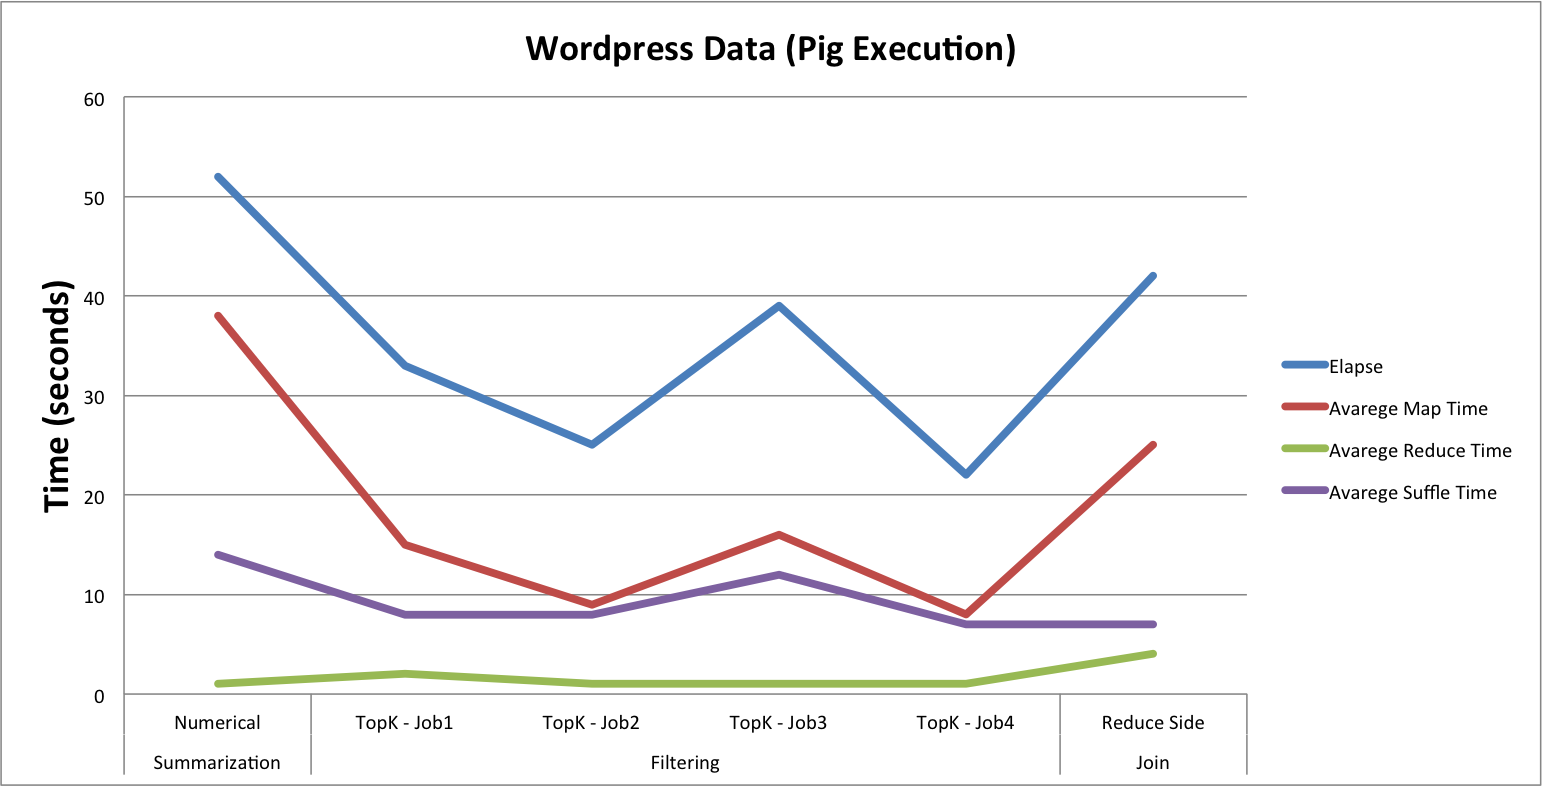
\includegraphics[width=0.49\textwidth]{figs/analysis-charts/pig/wordpress.png}}
   %add desired spacing between images, e. g. ~, \quad, \qquad etc. (or a blank line to force the subfig onto a new line)
  %~
  \\
  \subfloat[\textit{Webapps} Data]
  {\label{fig:pisp8}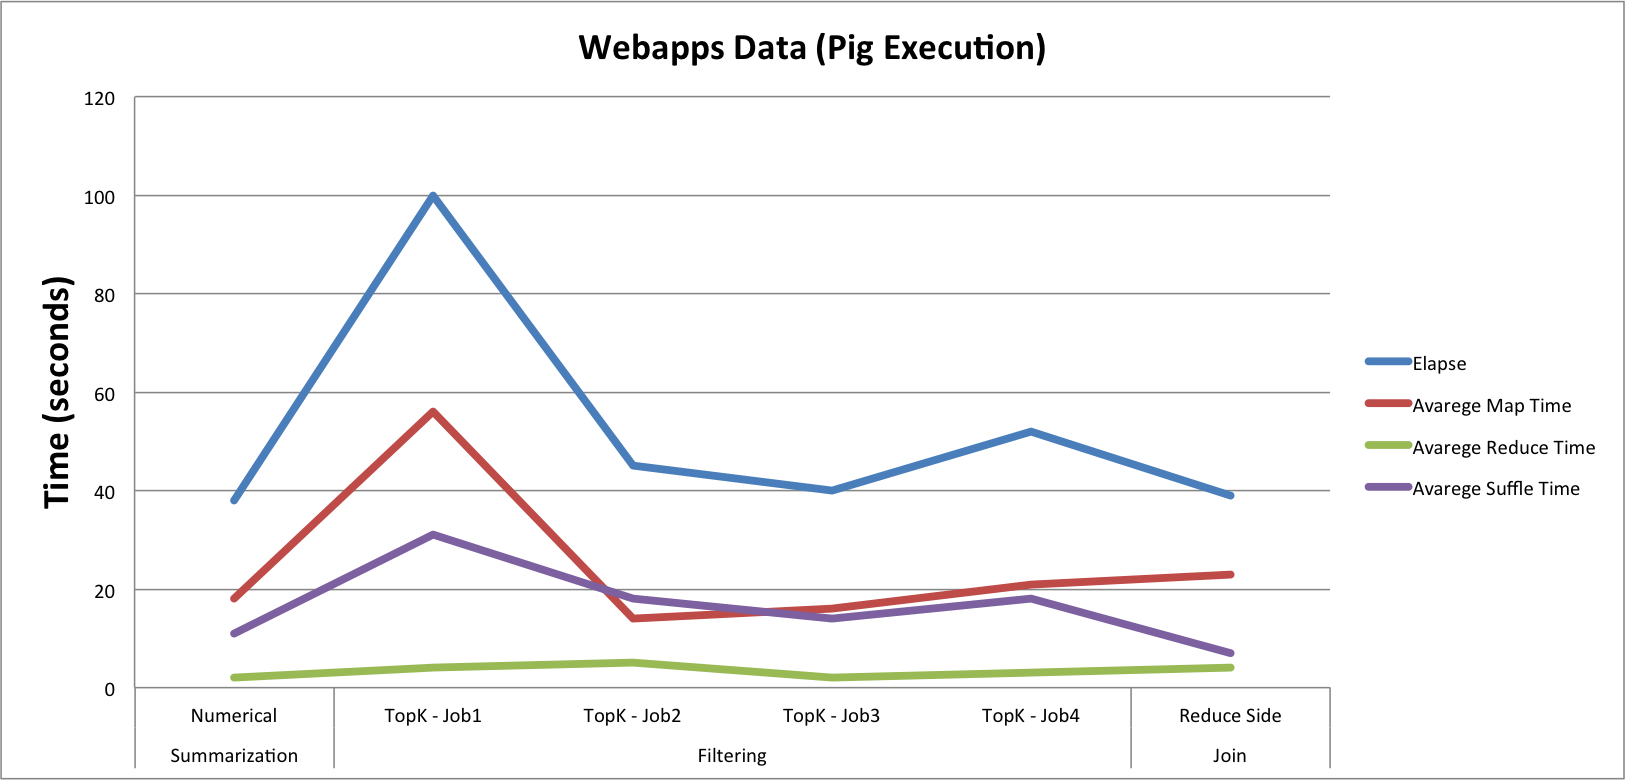
\includegraphics[width=0.5\textwidth]{figs/analysis-charts/pig/webapps.png}}
  ~ %add desired spacing between images, e. g. ~, \quad, \qquad etc. (or a blank line to force the subfig onto a new line)
 
  \caption{MapReduce Design Patterns Performance - Pig Execution.}
  \label{fig:pigexecution}
\end{figure}     
     
\begin{figure}[ht!]
 \centering 
  \subfloat[\textit{Ebooks} Data]
  {\label{fig:pisp6}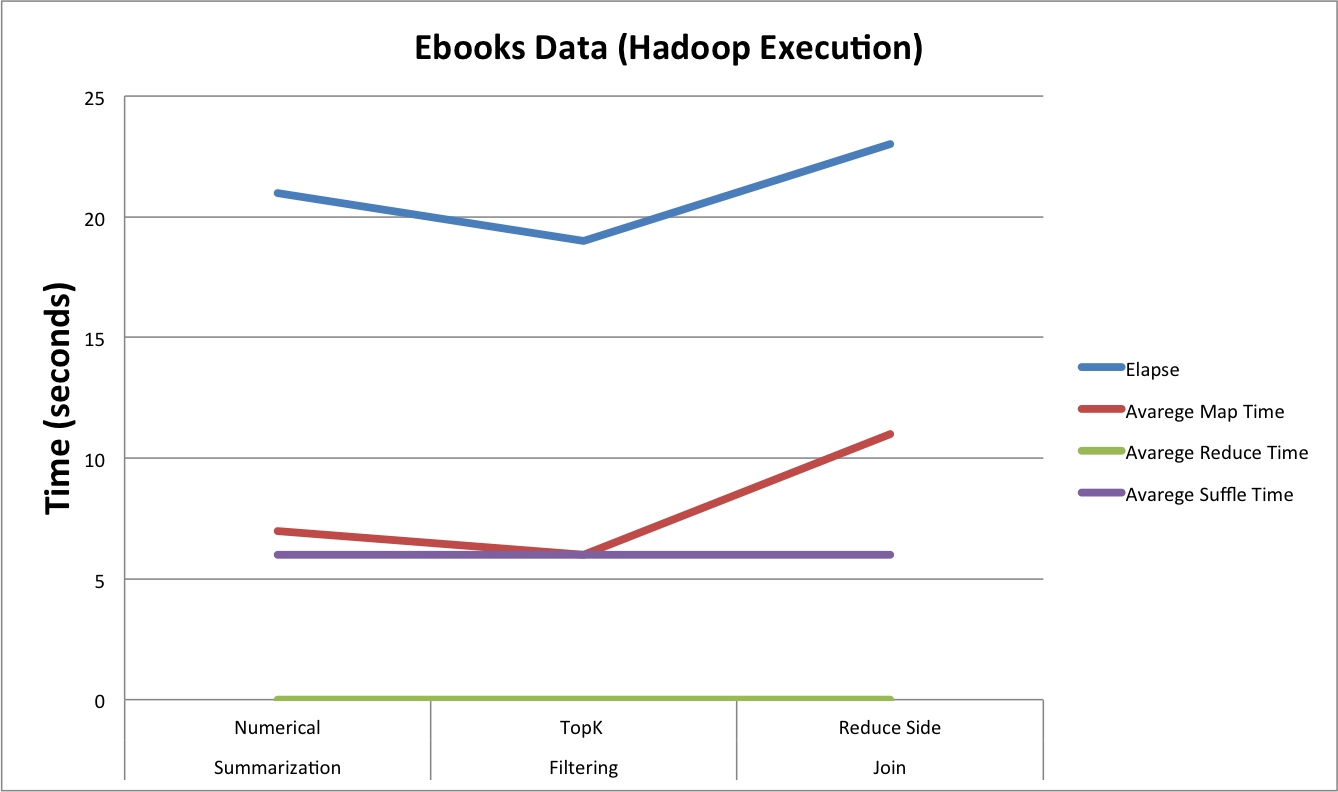
\includegraphics[width=0.456\textwidth]{figs/analysis-charts/hadoop/ebooks.png}}   
  \subfloat[\textit{Tex} Data]
  {\label{fig:pisp7}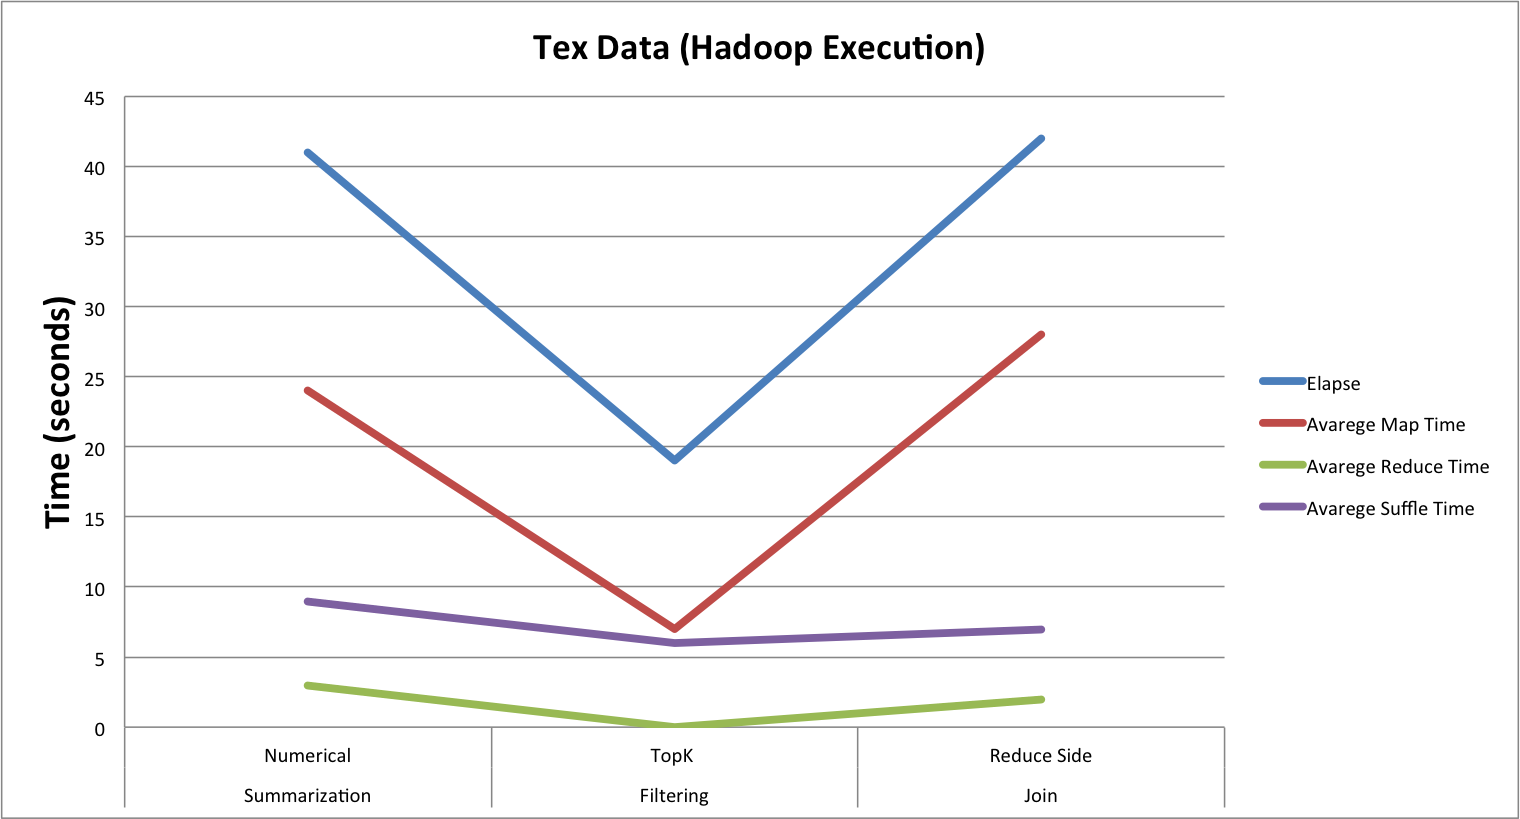
\includegraphics[width=0.5\textwidth]{figs/analysis-charts/hadoop/tex.png}}
   %add desired spacing between images, e. g. ~, \quad, \qquad etc. (or a blank line to force the subfig onto a new line)
  %~
  \\
  \subfloat[\textit{Serverfault} Data]
  {\label{fig:pisp6}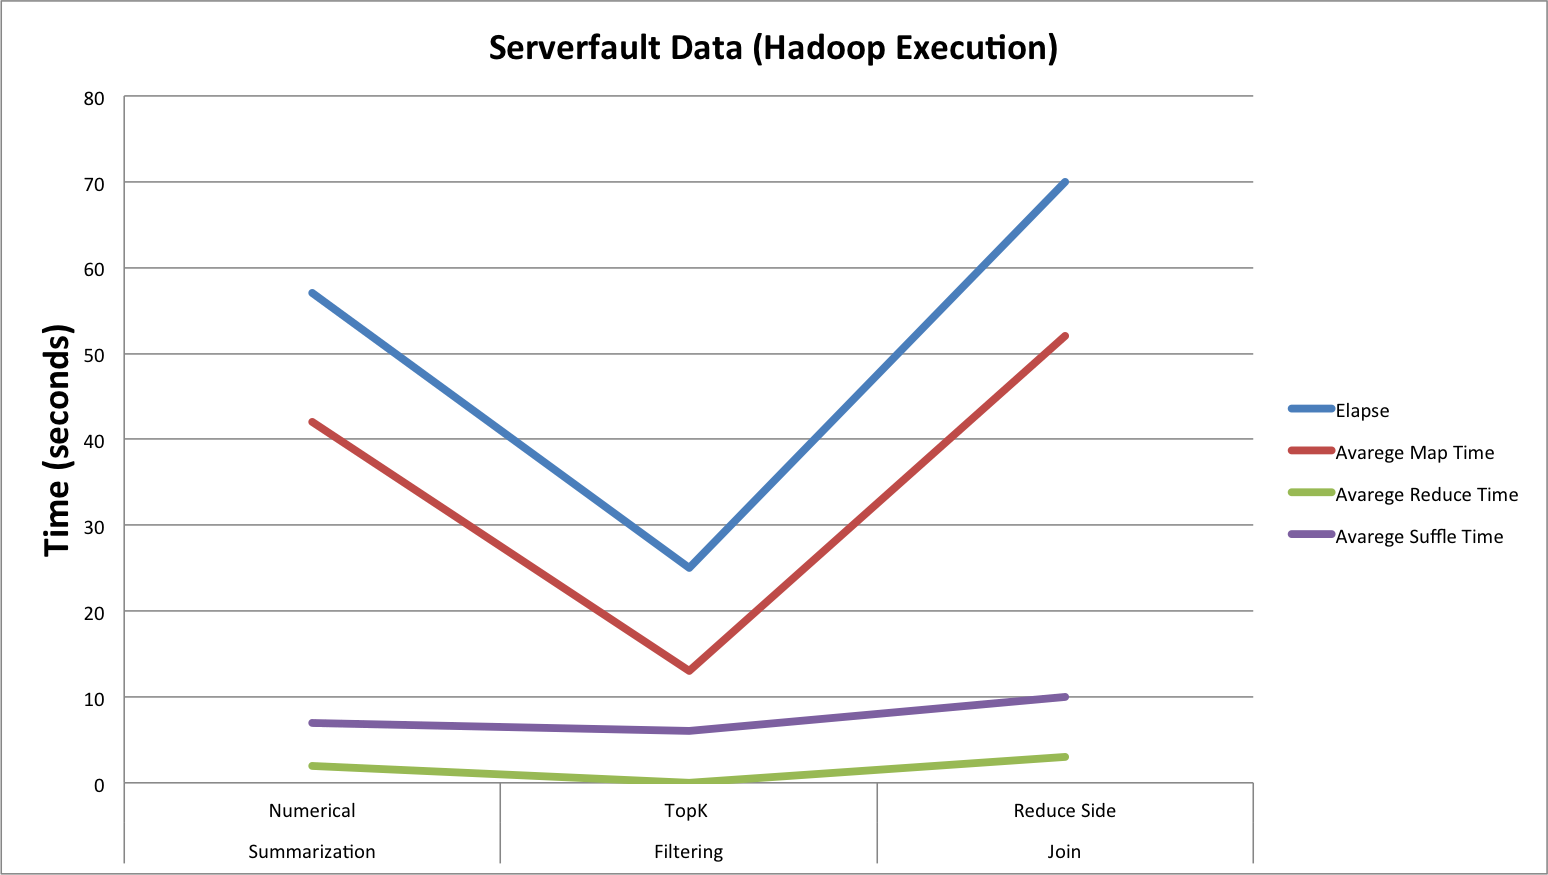
\includegraphics[width=0.485\textwidth]{figs/analysis-charts/hadoop/serverfault.png}}   
  \subfloat[\textit{Wordpress} Data]
  {\label{fig:pisp7}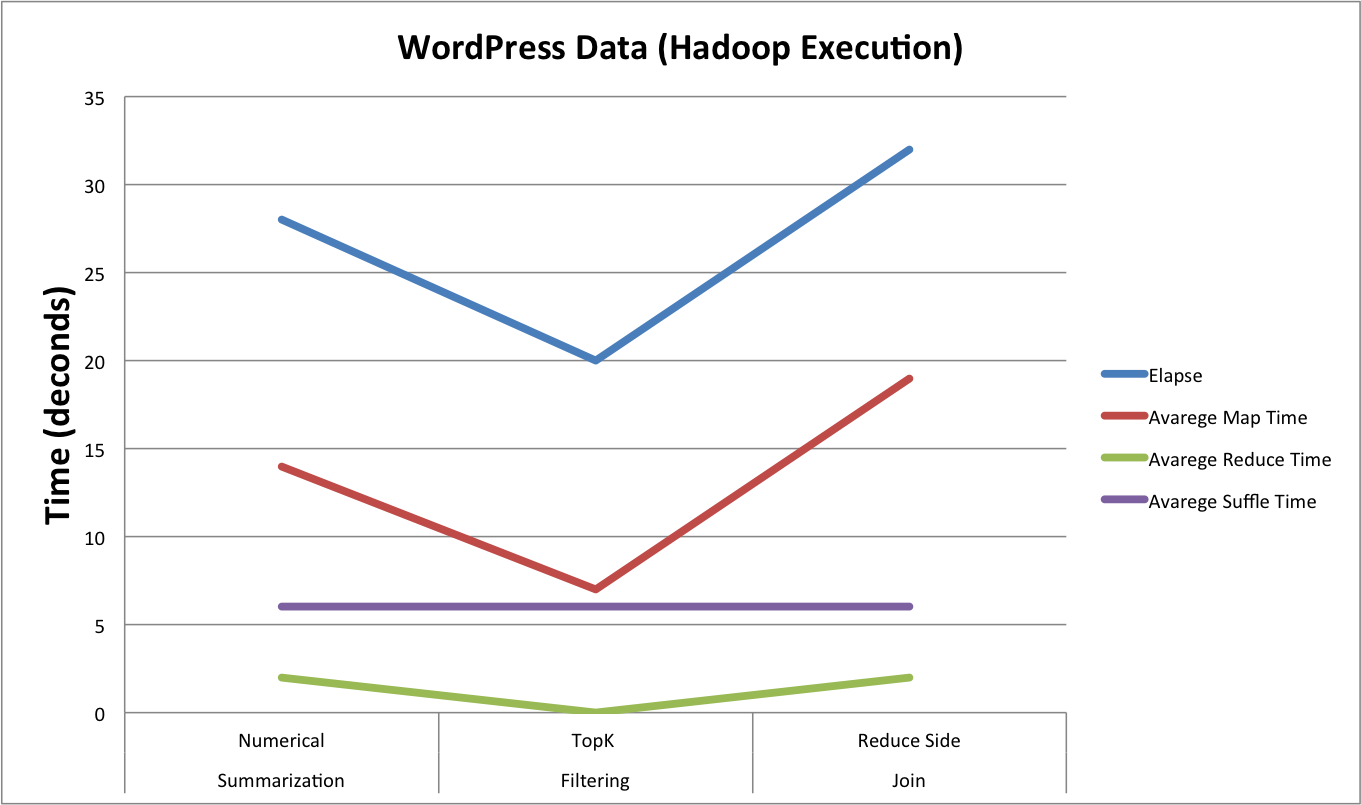
\includegraphics[width=0.466\textwidth]{figs/analysis-charts/hadoop/wordpress.png}}
   %add desired spacing between images, e. g. ~, \quad, \qquad etc. (or a blank line to force the subfig onto a new line)
  %~
  \\
  \subfloat[\textit{Webapps} Data]
  {\label{fig:pisp8}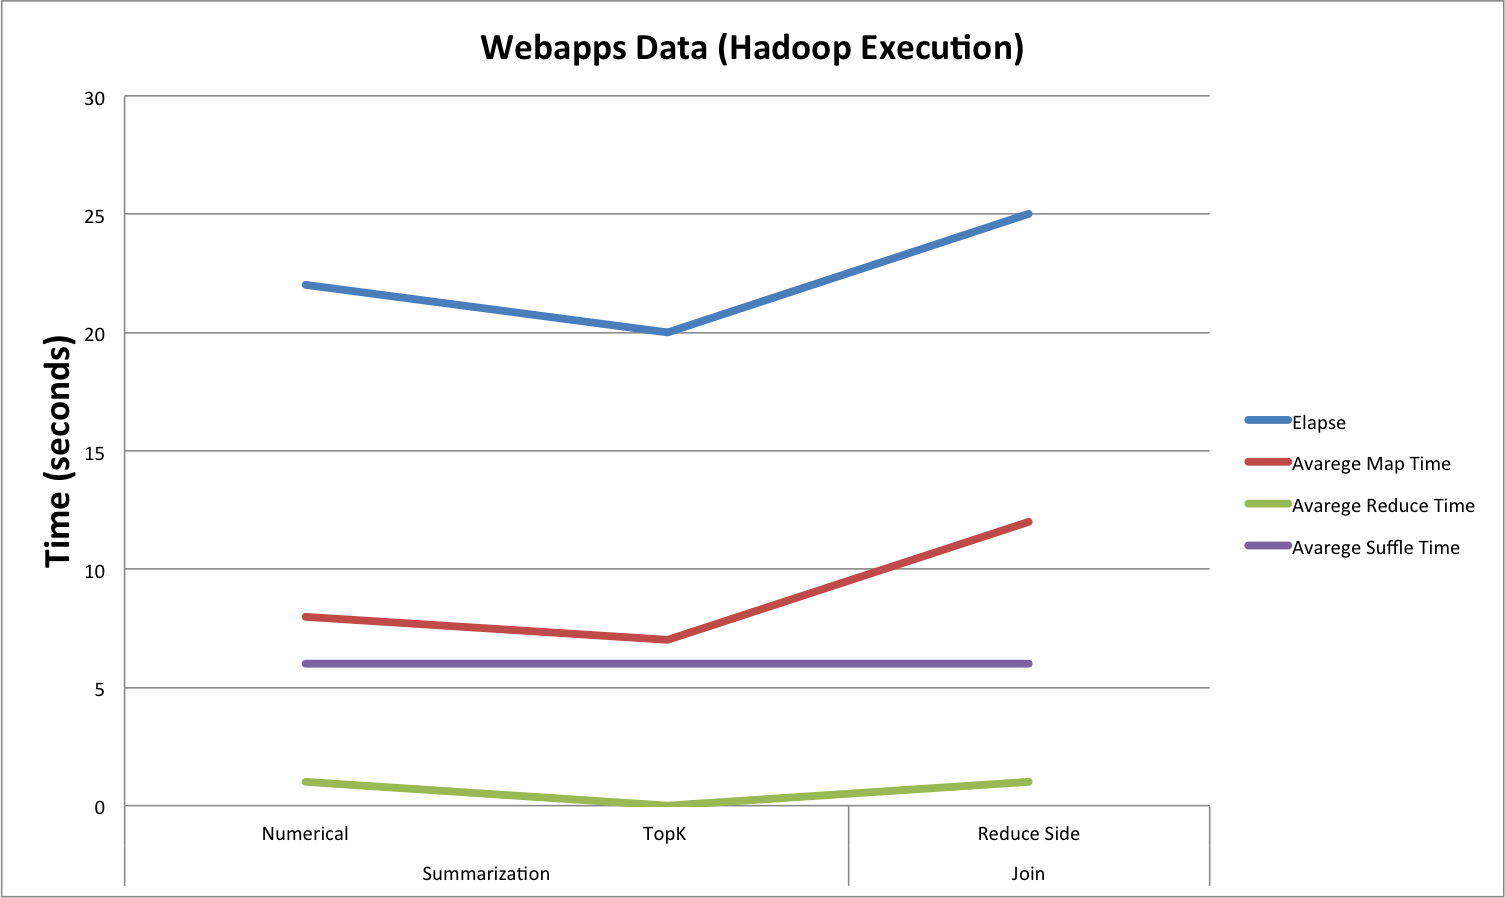
\includegraphics[width=0.5\textwidth]{figs/analysis-charts/hadoop/webapps.png}}
  ~ %add desired spacing between images, e. g. ~, \quad, \qquad etc. (or a blank line to force the subfig onto a new line)
  
  \caption{MapReduce Design Patterns Performance - Hadoop Execution.}
  \label{fig:hadoopexecution}
\end{figure}
   
   
       \begin{figure}[ht!]
 \centering 
 \subfloat[Mappers for Pig Execution]
  {\label{fig:mapperspig}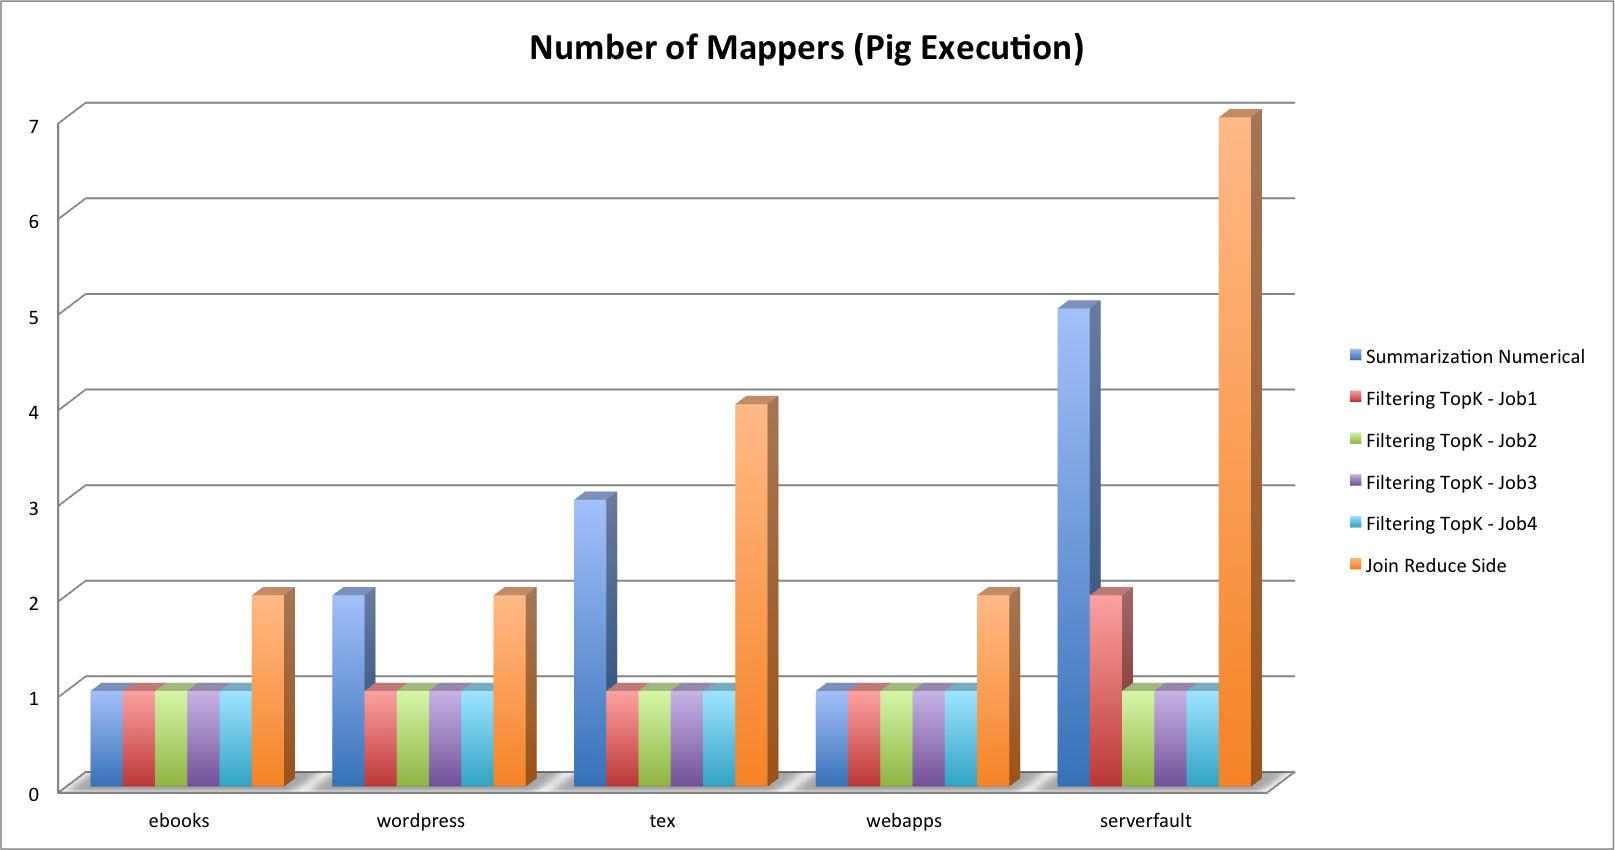
\includegraphics[width=0.6\textwidth]{figs/analysis-charts/pig/mappers.png}}
   %add desired spacing between images, e. g. ~, \quad, \qquad etc. (or a blank line to force the subfig onto a new line)
  %~
  \\
  \subfloat[Mappers for Hadoop Execution]
  {\label{fig:mappershadoop}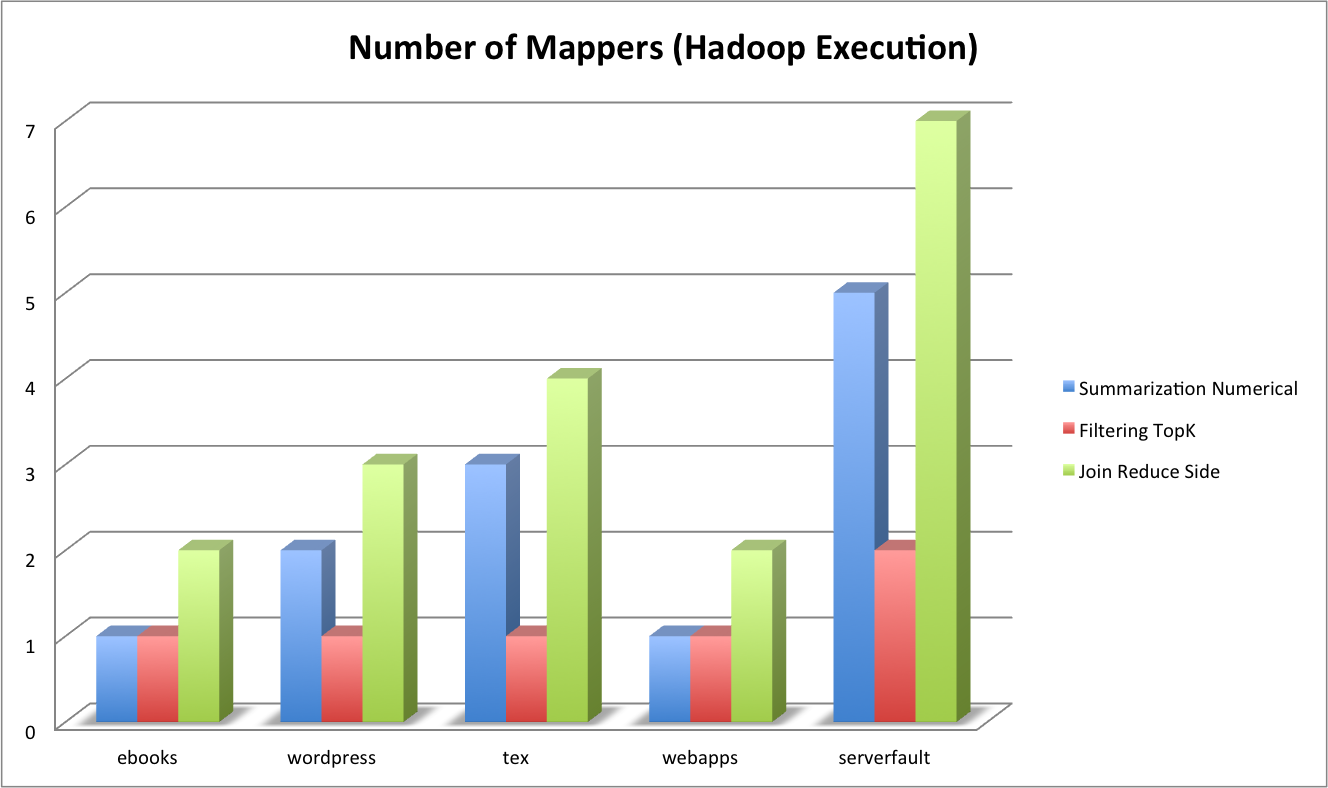
\includegraphics[width=0.6\textwidth]{figs/analysis-charts/hadoop/mappers.png}}
  ~ %add desired spacing between images, e. g. ~, \quad, \qquad etc. (or a blank line to force the subfig onto a new line)
 
  \caption{Number of Mappers - Pig and Hadoop Execution.}
  \label{fig:mappers}
\end{figure}
 
    